Uma base de dados experimentais se faz necessária para treinar e testar os modelos baseados em DL, fornecendo a experiência sobre o problema e permitindo o aprendizado por meio do ajuste dos parâmetros treináveis. Considerando este objetivo, a base dados considerada no escopo deste trabalho consiste no conjunto de imagens de validação da tarefa \emph{Fine-grained classification} do ILSVRC $2012$ \cite{ref:image-net}.

A base de dados experimentais adotada dispõe de um total de $50$ mil imagens de diferentes naturezas, as quais foram coletadas do \emph{website} Flickr e de outras plataformas semelhantes e rotuladas manualmente por ausência ou presença de $1000$ diferentes categorias \cite{ILSVRC}. Uma amostra das imagens contidas nesta base de dados pode ser vista na Figura \ref{fig:visaogeral}.

\begin{figure}[h]
	\centering
	\caption{Visão geral do conjunto de dados.}
	\label{fig:visaogeral}
	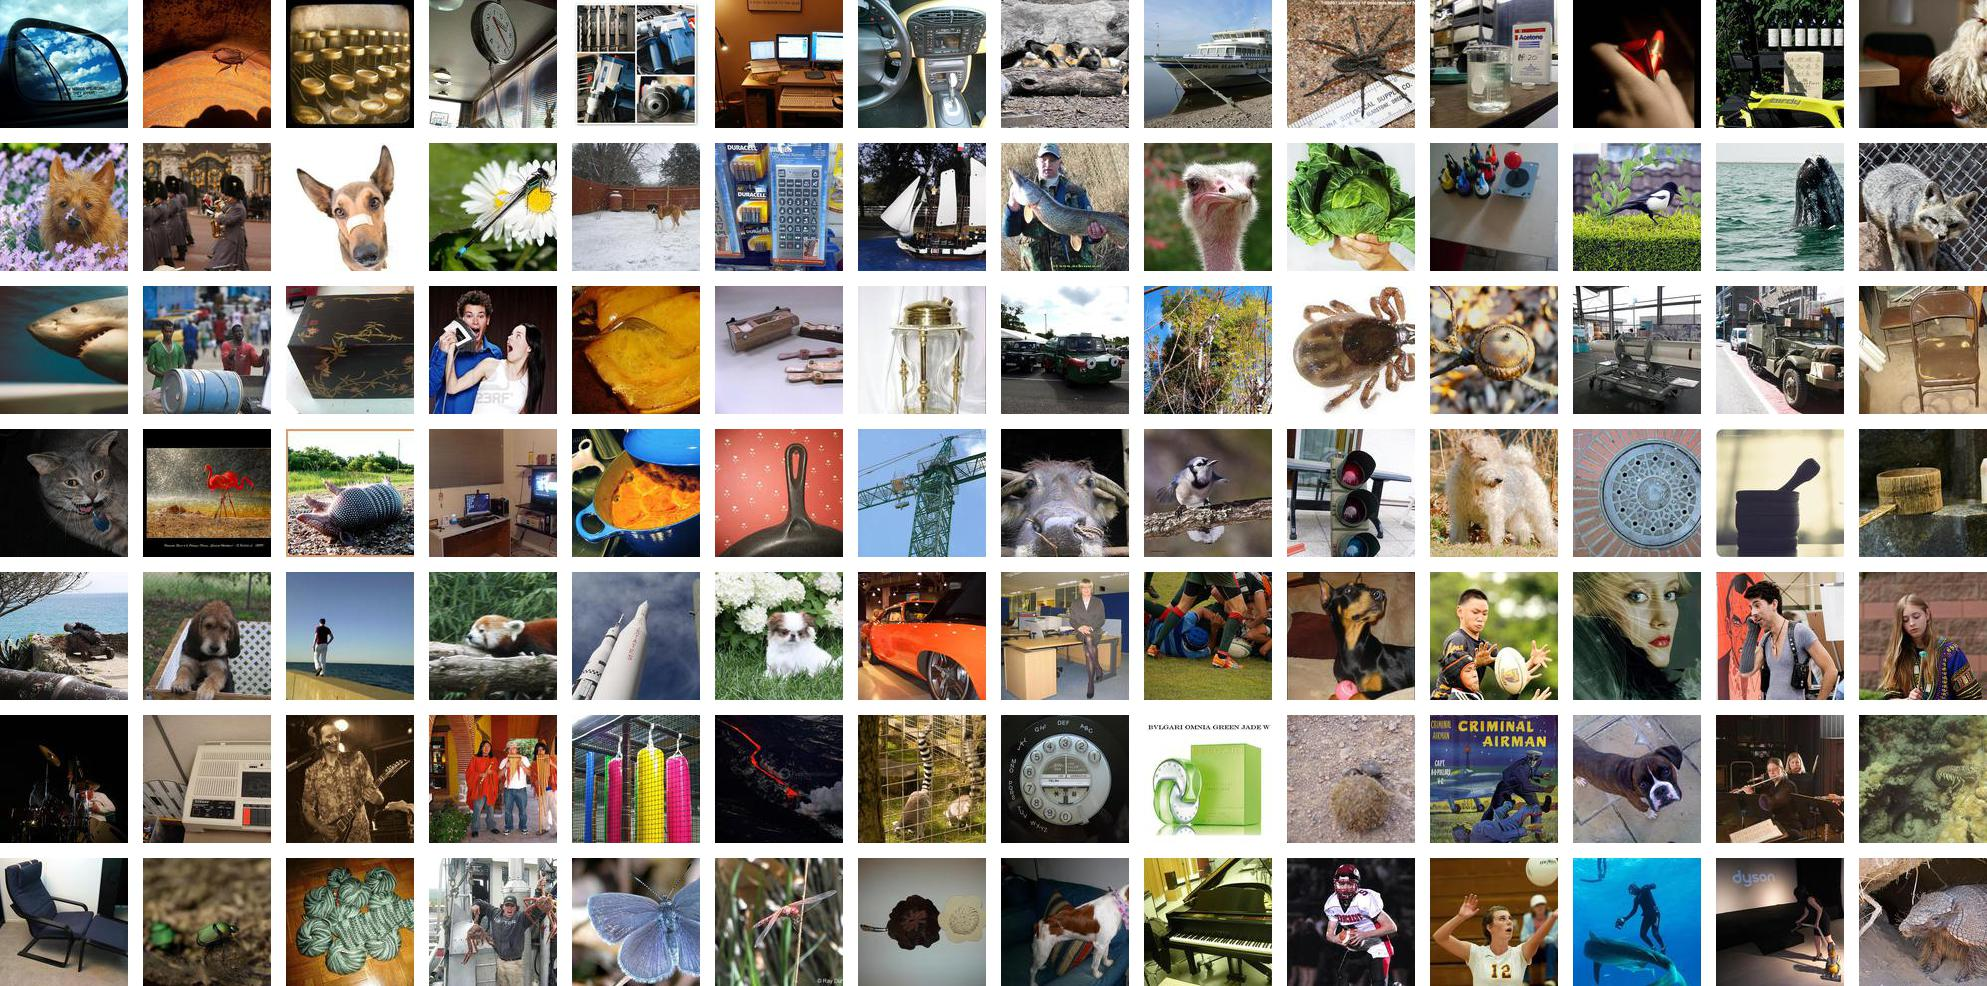
\includegraphics[width=1\textwidth]{./img/visaogeral}
\end{figure}

Esta base de dados foi escolhida por possuir uma quantidade de imagens favorável para o treinamento dos muitos parâmetros presentes nos modelos de DL e pelas imagens possuirem uma variedade de classes, o que caracteriza um conjunto de exemplos suficientemente representativo para a generalização em um cenário de colorização artificial. Embora haja conjuntos de imagens do ILSVRC de maior tamanho, este conjunto escolhido permite uma manipulação razoável dos dados, considerando os recursos computacionais disponíveis neste projeto.

Segundo a abordagem \emph{Holdout} de validação cruzada a ser adotada, conforme mencionado na Seção \ref{subsec:tarefa}, estas imagens serão particionadas em dois conjuntos: o de treinamento, contendo $35$ mil imagens, para ajuste dos parâmetros dos modelos; e o de testes, contendo as $15$ mil imagens remanescentes, para análise de desempenho.

Entretanto, antes de utilizar diretamente esta base de dados junto aos modelos de DL, as imagens precisaram de ajustes de pré-processamento, conforme detalhado na seção a seguir.
